\subsection{Relaxing mutual exclusivity to disjunction of systemic choices}
%\label{sec:system}
% exemplification of system
%TODO: Margaret Berry on Systems/Networks, David Butt on Systems, see citations in Rebekas's Thesis
%TODO: write email to Rebekah and ask about theory comparison literature

Fore example consider the polarity system represented in figure \ref{fig:polarity}. It contains two choices either positive or negative. And when one says it is positive one means not negative which is obvious and self evident how the two choices are mutually exclusive.

%\begin{figure}[H]
%	\centering
%	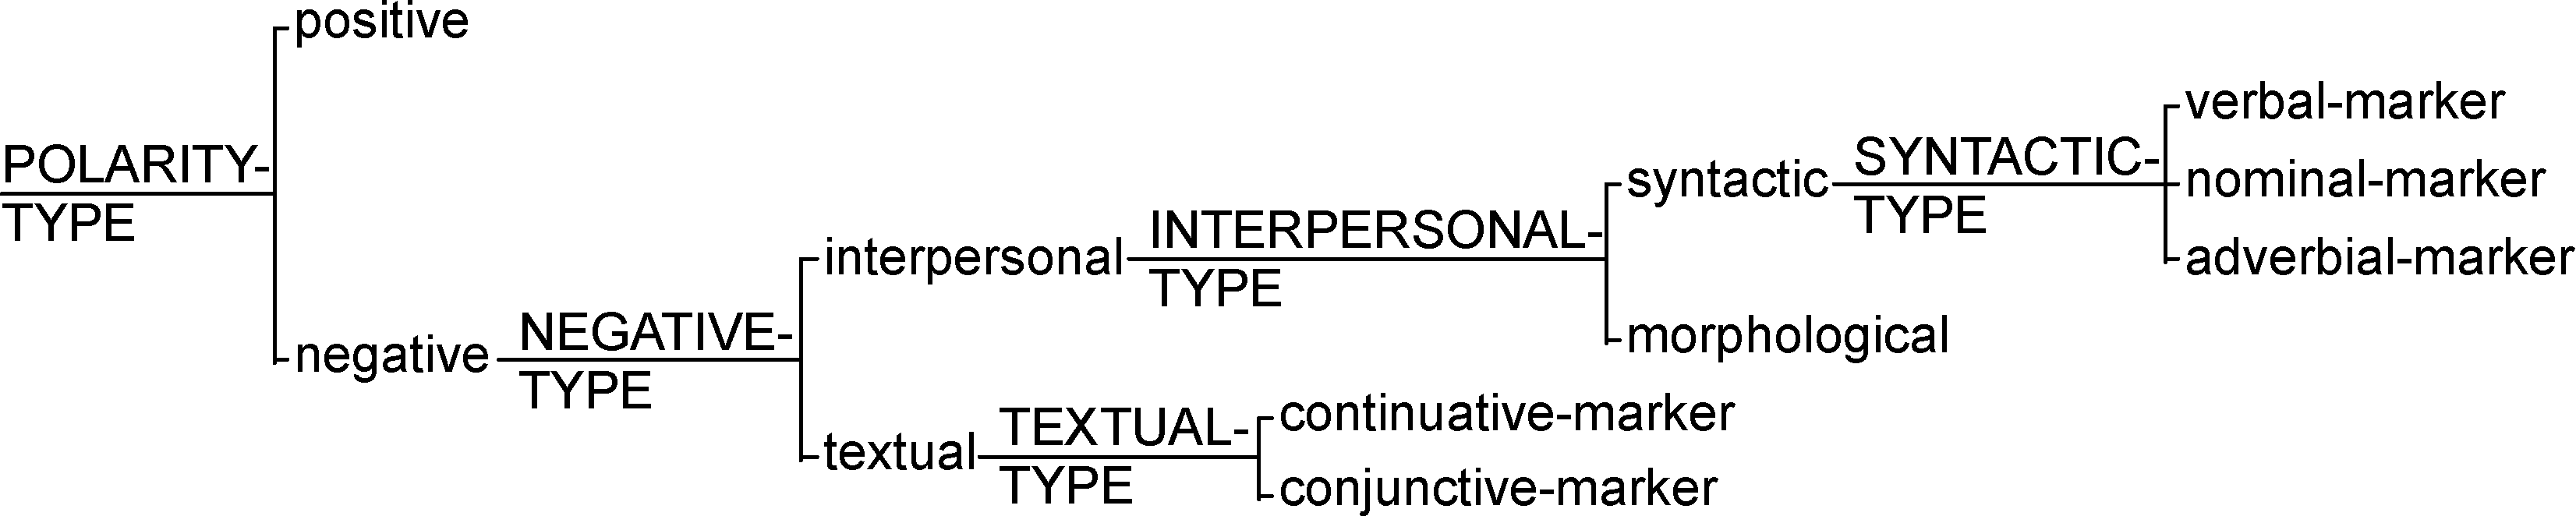
\includegraphics[width=\textwidth]{Figures/SFL-grammar/polarity-system.pdf}
%	\caption{System network of POLARITY}
%	\label{fig:polarity}
%\end{figure}

In language it may be often the case that a choice in a system may lead to re-entering the same system again to make another choice again forming this way recursive systems. Alternatively, we can say that a system allows multiple choices for the same unit. These perspectives are the sides of the same coin where the recursion perspective is useful for natural language generation while multiple choice perspective suits better the parsing task and next I explain why by continuing the discussion on polarity system. 

The negative polarity in English clauses can be realised in several ways: via a noun group with intrinsic negative polarity feature like \textit{``nobody''} (\ref{ex:neg1}), negation particle of the verb \textit{``n't''} (\ref{ex:neg2}) or adverb with intrinsic negative polarity (\ref{ex:neg3}). 

\begin{exe}
	\ex\label{ex:neg1} Nobody with any sense is going. 
	\ex\label{ex:neg2} I don't have to mow my lawn.
	\ex\label{ex:neg3} Never expect her to come back.
\end{exe}

Consider now, the cases of double negation from the example \ref{ex:double-negatives1} where two kinds of negations are realised in the same clause: the negation by verb particle \textit{``n't''} and the pronoun \textit{``nobody''}. 

\begin{exe}
	\ex \label{ex:double-negatives1}
	Nobody with any sense isn't going. 
	\ex \label{ex:double-negatives2} I don’t have nobody to mow my lawn.
\end{exe}

The systems can be recursive and thus choices are not always mutually exclusive. Even though the system network  clearly distinguishes one type of negation from another multiple negations can still occurring simultaneously. Note that this more delicate distinctions in kind of negation, still is a negation and for any of them it is impossible to co-occur with positive polarity. 
The issue here is not semantic about whether the clause is positive or negative but what kinds of grammatical choices can be identified within the clause. The problem of whether the double negation shall be interpreted as positive is not necessarily as relevant as the task of identifying the two instances of negation. 

Halliday states that the speaker makes only one choice from a system. If this rule is interpreted as two choices from the same system at a time being impossible then it clearly does not cover the recursive systems and needs weakening to accommodate border cases. I propose relaxing the constraint of \textit{mutual exclusivity} to \textit{disjunction}. Correspondingly, two types of systemic networks emerge differing by \textit{the relation among choices}: the original Hallidayan XOR systems (such as POLARITY TYPE in figure \ref{fig:polarity}) and the OR systems for accommodating cases of multiple feature selections (such as SYSTEMIC TYPE in the same figure).

